\documentclass{standalone}
\usepackage{pgfplots}
\pgfplotsset{compat=newest}
\begin{document}
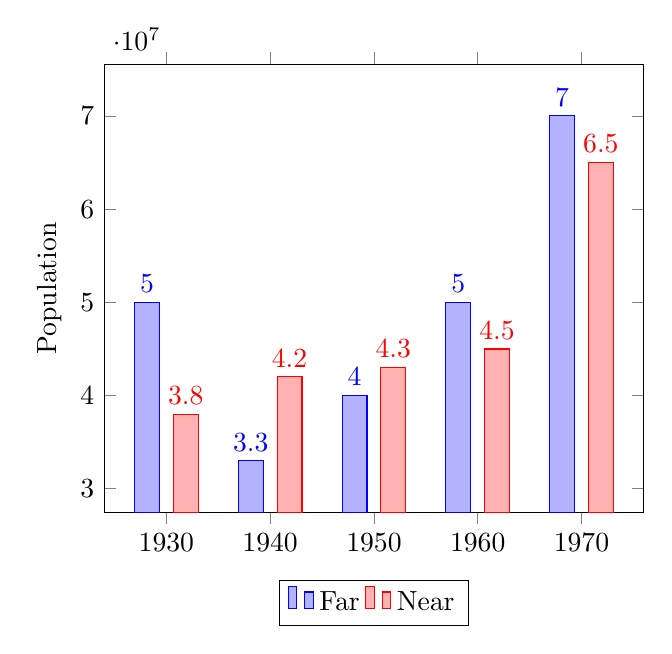
\begin{tikzpicture}
\begin{axis}[
	x tick label style={
		/pgf/number format/1000 sep=},
	ylabel=Population,
	enlargelimits=0.15,
	legend style={at={(0.5,-0.15)},
		anchor=north,legend columns=-1},
	ybar=5pt,% configures `bar shift'
	bar width=9pt,
	nodes near coords,
	point meta=y *10^-7 % the displayed number
]
\addplot 
	coordinates {(1930,50e6) (1940,33e6)
		 (1950,40e6) (1960,50e6) (1970,70e6)};
\addplot 
	coordinates {(1930,38e6) (1940,42e6) 
		(1950,43e6) (1960,45e6) (1970,65e6)};
\legend{Far,Near}
\end{axis}
\end{tikzpicture}
\end{document}
